\documentclass[nobib]{tufte-handout}
% \documentclass[fleqn,reqno,12pt]{article}

%========================================
% Packages
%========================================

\usepackage[nographicx, nohyperref, nosubcaption, nogb4e]{mfpackages}
\usepackage{mfenvironments}
\usepackage{mfcommands}
% for info boxes
\usepackage{newfloat, caption}
\DeclareCaptionType{InfoBox}


%========================================
% Bibliography
%========================================

\bibliography{references.bib}

%========================================
% General Layout Tweaks
%========================================

% \usepackage[margin=2cm]{geometry}

% Itemize
\renewcommand{\labelitemi}{\large{$\mathbf{\cdot}$}}    % itemize symbols
\renewcommand{\labelitemii}{\large{$\mathbf{\cdot}$}}
\renewcommand{\labelitemiii}{\large{$\mathbf{\cdot}$}}
\renewcommand{\labelitemiv}{\large{$\mathbf{\cdot}$}}
% Description
\renewcommand{\descriptionlabel}[1]{\hspace\labelsep\textsc{#1}}

% Figure Captions
\usepackage{caption} % use corresponding myfiguresize!
\setlength{\captionmargin}{20pt}
\renewcommand{\captionfont}{\small}
\setlength{\belowcaptionskip}{7pt} % standard is 0pt

%========================================
% Define colors and comment functions
%========================================

\usepackage{xcolor}
\definecolor{firebrick}{RGB}{178,34,34}
\definecolor{DarkGreen}{RGB}{34,178,34} 
\definecolor{DarkOrange}{RGB}{255,100,50}
\renewcommand{\mf}[1]{\textcolor{firebrick}{[mf: #1]}}  
\newcommand{\tr}[1]{\textcolor{DarkOrange}{[tr: #1]}}  
%========================================
% Configuring the R code presentation
%========================================

\usepackage{courier}
\usepackage{listings}
\usepackage{color}
% the following defines the layout for the R code
\lstset{ %
  language=R,                     % the language of the code
  basicstyle=\footnotesize\ttfamily, % size and type of the fonts that are used for the code
  numbers=left,                   % where to put the line-numbers
  numberstyle=\tiny\color{gray},  % the style that is used for the line-numbers
  stepnumber=1,                   % the step between two line-numbers. If it's 1, each line
                                  % will be numbered
  numbersep=5pt,                  % how far the line-numbers are from the code
  backgroundcolor=\color{white},  % choose the background color. You must add \usepackage{color}
  showspaces=false,               % show spaces adding particular underscores
  showstringspaces=false,         % underline spaces within strings
  showtabs=false,                 % show tabs within strings adding particular underscores
  frame=single,                   % adds a frame around the code
  rulecolor=\color{black},        % if not set, the frame-color may be changed on line-breaks within not-black text (e.g. commens (green here))
  tabsize=2,                      % sets default tabsize to 2 spaces
  captionpos=b,                   % sets the caption-position to bottom
  breaklines=true,                % sets automatic line breaking
  breakatwhitespace=false,        % sets if automatic breaks should only happen at whitespace
  title=\lstname,                 % show the filename of files included with \lstinputlisting;
                                  % also try caption instead of title
  keywordstyle=\color{blue},      % keyword style
  commentstyle=\color{DarkGreen}, % comment style
  stringstyle=\color{DarkOrange}, % string literal style
  escapeinside={\%*}{*)},         % if you want to add a comment within your code
  morekeywords={*, ...}            % if you want to add more keywords to the set
}

% this is for showing the R output
\lstnewenvironment{rc}[1][]{\lstset{language=R}}{}

% this is for inline R code
\newcommand{\ri}[1]{\lstinline{#1}}  %% Short for 'R inline'


%========================================
% Article Header 
%========================================


\title{Hands-on non-technical tutorial for Bayesian mixed effects regression}
\author{Michael Franke \& Timo Roettger}
\date{}

%========================================
% Article Body
%========================================

\begin{document}
\maketitle

\begin{abstract}
  \noindent Generalized linear mixed models are very versatile and handy tools for statistical inference. Bayesian approaches to applying these models have recently become increasingly popular. This tutorial provides an accessible, non-technical introduction to the use and feel of Bayesian mixed effects regression models. The focus is on data from a factorial-design experiment. \\
  
  \medskip
  
  \noindent \textbf{This tutorial should take you about 1 hour.}
\end{abstract}

\section{Motivation \& intended audience}

This tutorial provides a very basic introduction to Bayesian regression modeling using R \citep{Manual}. We wrote this tutorial with a particular reader in mind. If you have used R before and if you have a basic understanding of linear regression and now you want to find out what a Bayesian approach has to offer, this tutorial is for you. In comparison to other introductions \citep[e.g.][]{SorensenHohensteinb2016:Bayesian-linear}, this tutorial remains very conceptual. We don’t want to ``sell Bayes'' to you, and we do not want to scare you away with mathematical details. We just want to give you an impression of how a Bayesian regression analysis looks and feels. So no reason to be afraid! But also: no reason to be bored, because we \emph{will} cover all the essential concepts and we \emph{will} explain how to run and interpret the output of a Bayesian regression analysis using the wonderful R package \texttt{brms} written by Paul \citet{buerkner2016brms}.

If you don’t have any experience with regression modeling, you will probably still be able to follow but you might also want to consider doing a crash course. To bring you up to speed, we recommend the excellent two-part tutorial by Bodo \citet{Winter2013:Linear-models-a} on mixed effects regression in a non-Bayesian ---a.k.a.~classical or frequentist--- paradigm. In a sense, this tutorial could be considered part three of Bodo's nice and lofty introduction. We will, for example use the same data set.

This tutorial contains text boxes (with a gray background) which contain additional background information on some topics.
The information is sometimes a bit technical but never absolutely necessary for understanding the main ideas.
So, feel free to read or skip any of the text boxes to suit your needs.

To follow this tutorial, you should have R installed on your computer (\url{https://www.r-project.org}).
Unless you already have a favorite editor for tinkering with R scripts, we recommend to try out RStudio (\url{https://www.rstudio.com}).
You will also need some packages,
\marginnote{Remember that you can install a package called \texttt{XYZ} with the command \texttt{install.packages('XYZ')}.}
which you can import with the following code:
\marginnote{If you do not want to copy-paste, all code and data for this tutorial is also
  available for download here:
  \url{https://github.com/michael-franke/bayes_mixed_regression_tutorial}}
\marginnote{We wrote a small R package with convenience functions for this tutorials, the
  \texttt{faintr} package, which the code in this code box attempts to download and install (like 20).}

\begin{minipage}[]{\textwidth}
\begin{lstlisting}[language=R]
#####################################################
## package includes and options
#####################################################

# package for convenience functions (e.g. plotting)
library(tidyverse)

# package for Bayesian regression modeling
library(brms)
# option for Bayesian regression models: use all available cores for parallel computing
options(mc.cores = parallel::detectCores())

# package for function 'std.error' to obtain standard errors
library(plotrix)

# package to allow installation from github
library(devtools)

# package with convenience function for Bayesian regression models for factorial designs
install_github('michael-franke/bayes_mixed_regression_tutorial/faintr') # install from GitHub
library(faintr)

# package to navigate to your source folder
library(rstudioapi)

## Getting the path of your current open file
current_path = rstudioapi::getActiveDocumentContext()$path 
setwd(dirname(current_path))
\end{lstlisting}
\end{minipage}

\section{Data, research questions \& hypotheses}
\label{sec:data}

Imagine we are experimental researchers. Therefore, we collect data to answer questions of
interest about how nature works. For example, we might want to know whether voice pitch differs across female and male speakers, and whether it differs across social contexts (say: informal and polite contexts). --- To answer our questions, we come up with a nifty experimental design, we lure a group of people into the lab, we ask them to say different words in different social contexts, we record their voices, and extraxt some numbers from these recordings, for example, the pitch values of their voices. We then want to find out whether our data provide evidence for any assumed relationships. So far so good.

In this tutorial, we are looking at data just like this
\citep[following][]{Winter2013:Linear-models-a}\marginnote{The data is originally from research
presented by \citet{WinterGrawunder2012:The-Phonetic-Pr}}. To load the data into your session,
run the following code:
\marginnote{If you are familiar with the previous tutorials by \citet{Winter2013:Linear-models-a}, it might help to know that we massaged the data a bit, e.g., renaming of variables or removing a line with missing data, so it differs slightly from the data set used in earlier tutorials by Winter.}

\medskip


\begin{minipage}[]{\textwidth}
\begin{lstlisting}[language=R]
  # load the data into variable 'politedata'
 politedata = read_csv('https://raw.githubusercontent.com/michael-franke/bayes_mixed_regression_tutorial/master/code/politeness_data.csv') 
\end{lstlisting}
\end{minipage}

\vspace*{-0.5cm}

\noindent Type \ri{head(politedata)} and you should see the first lines of the imported
data:\marginnote{Here, we show only part of the output that you might see when executing this
  command.}

\medskip

\begin{minipage}[]{\textwidth}
\begin{rc}
> head(politedata)
   subject gender sentence context pitch
   <chr>   <chr>  <chr>    <chr>   <dbl>
 1 F1      F      S1       pol      213.
 2 F1      F      S1       inf      204.
 3 F1      F      S2       pol      285.
 4 F1      F      S2       inf      260.
 5 F1      F      S3       pol      204.
\end{rc}
\end{minipage}


\medskip

\noindent This data set contains information about different subjects, with an anonymous identifier stored in variable \texttt{subject}.
Because voice pitch is highly dependent on gender, we stored whether our subjects are F(emale) or M(ale) in variable \texttt{gender}.
Subjects produced different sentences (stored in variable \texttt{sentence}), and the experiment manipulated whether the sentence was produced in a polite or an informal context.
This is indicated by the variable \texttt{context}. Crucially, each row contains a measurement of pitch in Hz stored in variable \texttt{pitch}.

Often, we are interested in comparing a \textbf{dependent variable} (here \texttt{pitch})
across different conditions or groups, i.e. \textbf{independent variables} (here \texttt{gender} and \texttt{context}). Before our data collection,
we might have formulated concrete predictions about the relationship between the dependent
variable and independent variables. For example, we might have formulated the following three
hypotheses:\marginnote{Notice that our hypotheses are formulated explicitly as comparisons of
  means / averages. The statistical model we will use indeed compares means, and this is common
  practice, albeit a particular assumption worth flagging. Very commonly this assumption is implicit and so you could encounter H1 formulated flatly as, e.g.,
  ``Female speakers' pitch is lower in polite than informal contexts.'' }

\begin{enumerate}[{H}1:]
\item Female speakers have a lower average pitch in polite than in informal contexts.
\item Male speakers have a lower average pitch in polite than in informal contexts.
\item Male speakers have a lower average pitch in informal than female speakers have in polite contexts.
\end{enumerate}

\section{Exploring the data visually}

To get a first idea of possible relationships in our data, let's plot
them.\marginnote{Extensive plotting is always recommended to start data analysis. You need to
  know your data inside out. Pictures often reveal complex relationships much better than
  numbers can.} Figure~\ref{fig:BasicPlotData_data} displays the mean pitch values for each
sentence (semi-transparent points) across gender and attitude. The solid points indicate the
mean pitch values across gender and context. Looking at the plot, we can see that pitch values
from female speakers are generally higher than values from male speakers (points in left column
are higher than in the right column). We also see that pitch values in the informal context
condition are slightly higher than those in the polite context condition (blue points are
slightly higher than orange points).\marginnote{The code needed to generated the picture in
  Figure~\ref{fig:BasicPlotData_data} is not reproduced here, but included in the script in the
  resources for this tutorial: \url{https://github.com/ michael- franke/bayes_mixed_
    regression_tutorial}}

\begin{figure}[t]
  \centering
    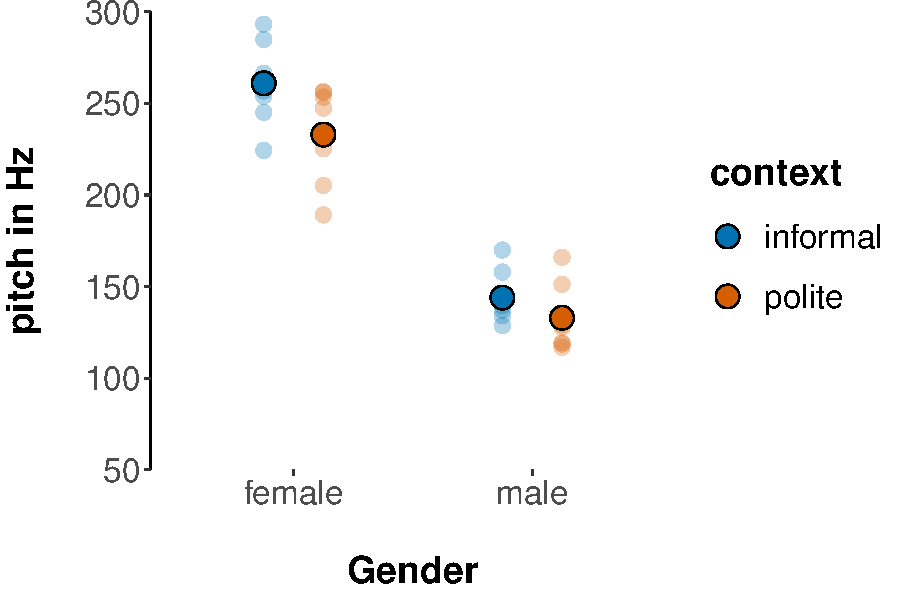
\includegraphics[width = \textwidth]{pics/basic_data_plot.pdf}
    \caption{Basic plot of the data.}
     \label{fig:BasicPlotData_data}
\end{figure}

Based on keen eye-balling, we might want to shout: ``Ha! The data confirm all of our
hypotheses!'' But, of course, we need to be more careful. We would like to translate the data
into an expression of \textbf{evidence}: does the data provide evidence for our research
hypotheses? Or are the observable differences to meager? -- Also, notice that there is quite a
lot of variability between different sentences (the semi-transparent dots). For example, some
values from the informal condition for female speakers (blue points in left column), are lower
than their corresponding polite counterparts. Similarly, there could be quite some differences
between individual speakers. Consequently, what we want is precise estimates of potential
differences between conditions, alongside a measure of certainty around these estimates.

\begin{figure}[h]
  \centering
    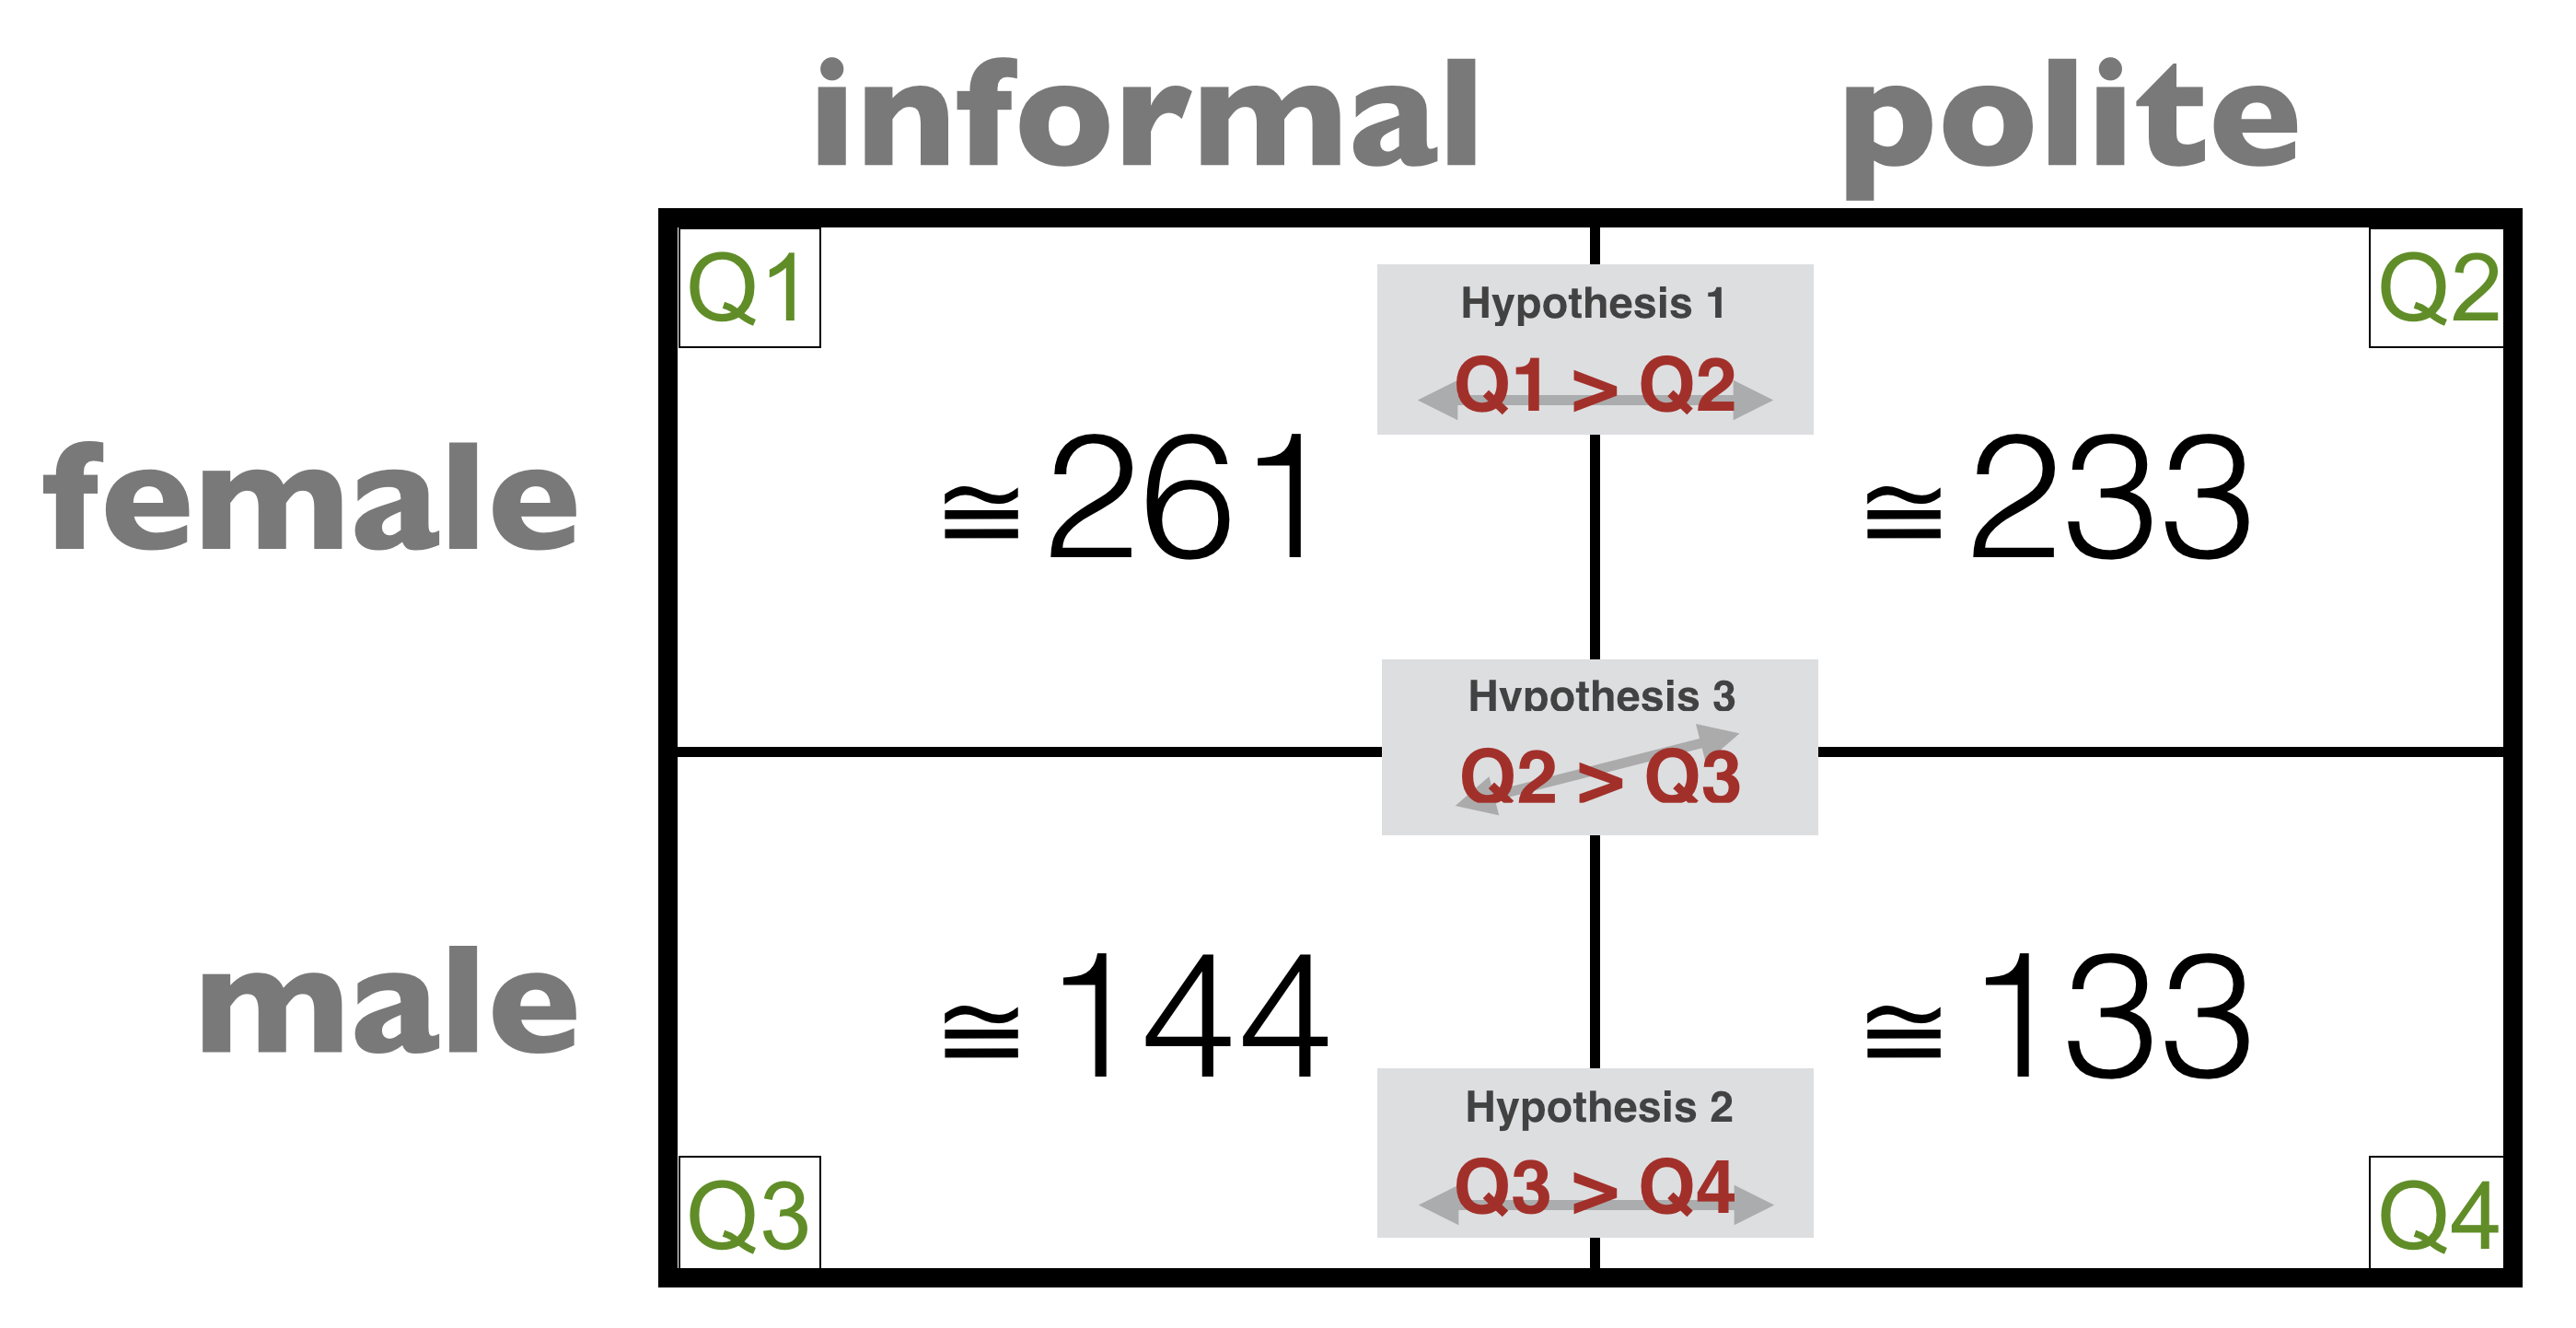
\includegraphics[width = \textwidth]{pics/table_mean_hypotheses.png}
    \caption{Means of each design cell, together with research hypotheses as statements about ordinal relations between cell means.}
    \label{fig:BasicPlotData_table}
\end{figure}

\section{A regression model for our data}

Another way of looking at the data in connection with our research hypotheses is in Figure~\ref{fig:BasicPlotData_table}. Each cell represent one unique combination of the gender and the context factor, and the table shows the mean pitch value for each cell.\marginpar{In technical terms, this table is the \textbf{design matrix} of our experiment. We have two factors of interest \texttt{context} and \texttt{gender}, each with two levels. The table shows each combination of levels of all relevant factors. The cells in this table are therefore also called \textbf{design cells}.}
Our hypotheses can be related to the comparison between some of these cell-based means.
H1 makes a statement about the comparison between cells 1 and 2 (the context effect for female speakers); H2 makes a statement about cells 3 and 4 (the context effect for male speakers); and H3 makes a statement about cells 2 and 3 (the difference between informal male speakers and polite female speakers).

One way of testing our hypotheses using a Bayesian approach to data analysis, is to ask whether, given the data, the relevant differences between cell means are credibly different from zero. This is, as we will see below, jargon for asking whether, given the data, we should believe that the relevant cell means are different. The important bit about the Bayesian approach is in the ``credibly different'' and the ``should believe''. The Bayesian approach is about updating beliefs (expressed as probability distributions). This may appear scary or technically involved. But at the end of the day the intuitions captured by this approach are arguably very natural, and perhaps easier to understand that the motivations underlying other approaches to data analysis. Let's try to tackle this step by step.

First, let us look at the \textbf{regression model} we want to use.\marginnote{While other
  approaches to data analysis might stress the application of statistical tests, a Bayesian
  approach puts more emphasis on the fact that all statistical inference resolves around a
  statistical model; which is usually an assumption about how the data was generated. This
  model is, almost certainly, always false. But even a false model can be useful; conclusions
  based on a false model can be meaningful and insightful.} As usual in regression models for
factorial designs, like the present one, we assume that pitch values observed in each cell are
samples from some normal distribution, where each cell $c_i$ has its own mean $\mu_i$. We are
ultimately interested in the probability of the proposition that one cell's mean is bigger than
another's, i.e., whether $\mu_i > \mu_j$. Since the latter is equivalent to $\mu_i - m_j > 0$,
and since, let's say, it is easier to test whether a value is bigger than zero, we can encode
the cell means like in Figure~\ref{fig:coefficients_table}. This encoding scheme assumes that
there is a \textbf{reference level} for each factor. Here it is the level \texttt{female} for
the factor \texttt{gender} and the level \texttt{informal} for the factor
\texttt{context}.\marginnote{This is so-called \textbf{dummy coding} of the regression
  coefficients. Other coding schemes exist.} All cell means can then be expressed in terms of
differences between the \textbf{intercept} $\beta_0$ which is the cell mean of the cell where
all factors have their reference levels (here, the cell mean for pitch of female speakers in
informal contexts) and deviations from this \textbf{reference cell} for each individual factor
($\beta_{\text{male}}$, and $\beta_{\text{polite}}$), and a so-called \textbf{interaction term}
$\beta_{\text{pol\&male}}$.

\begin{figure}[h]
  \centering
    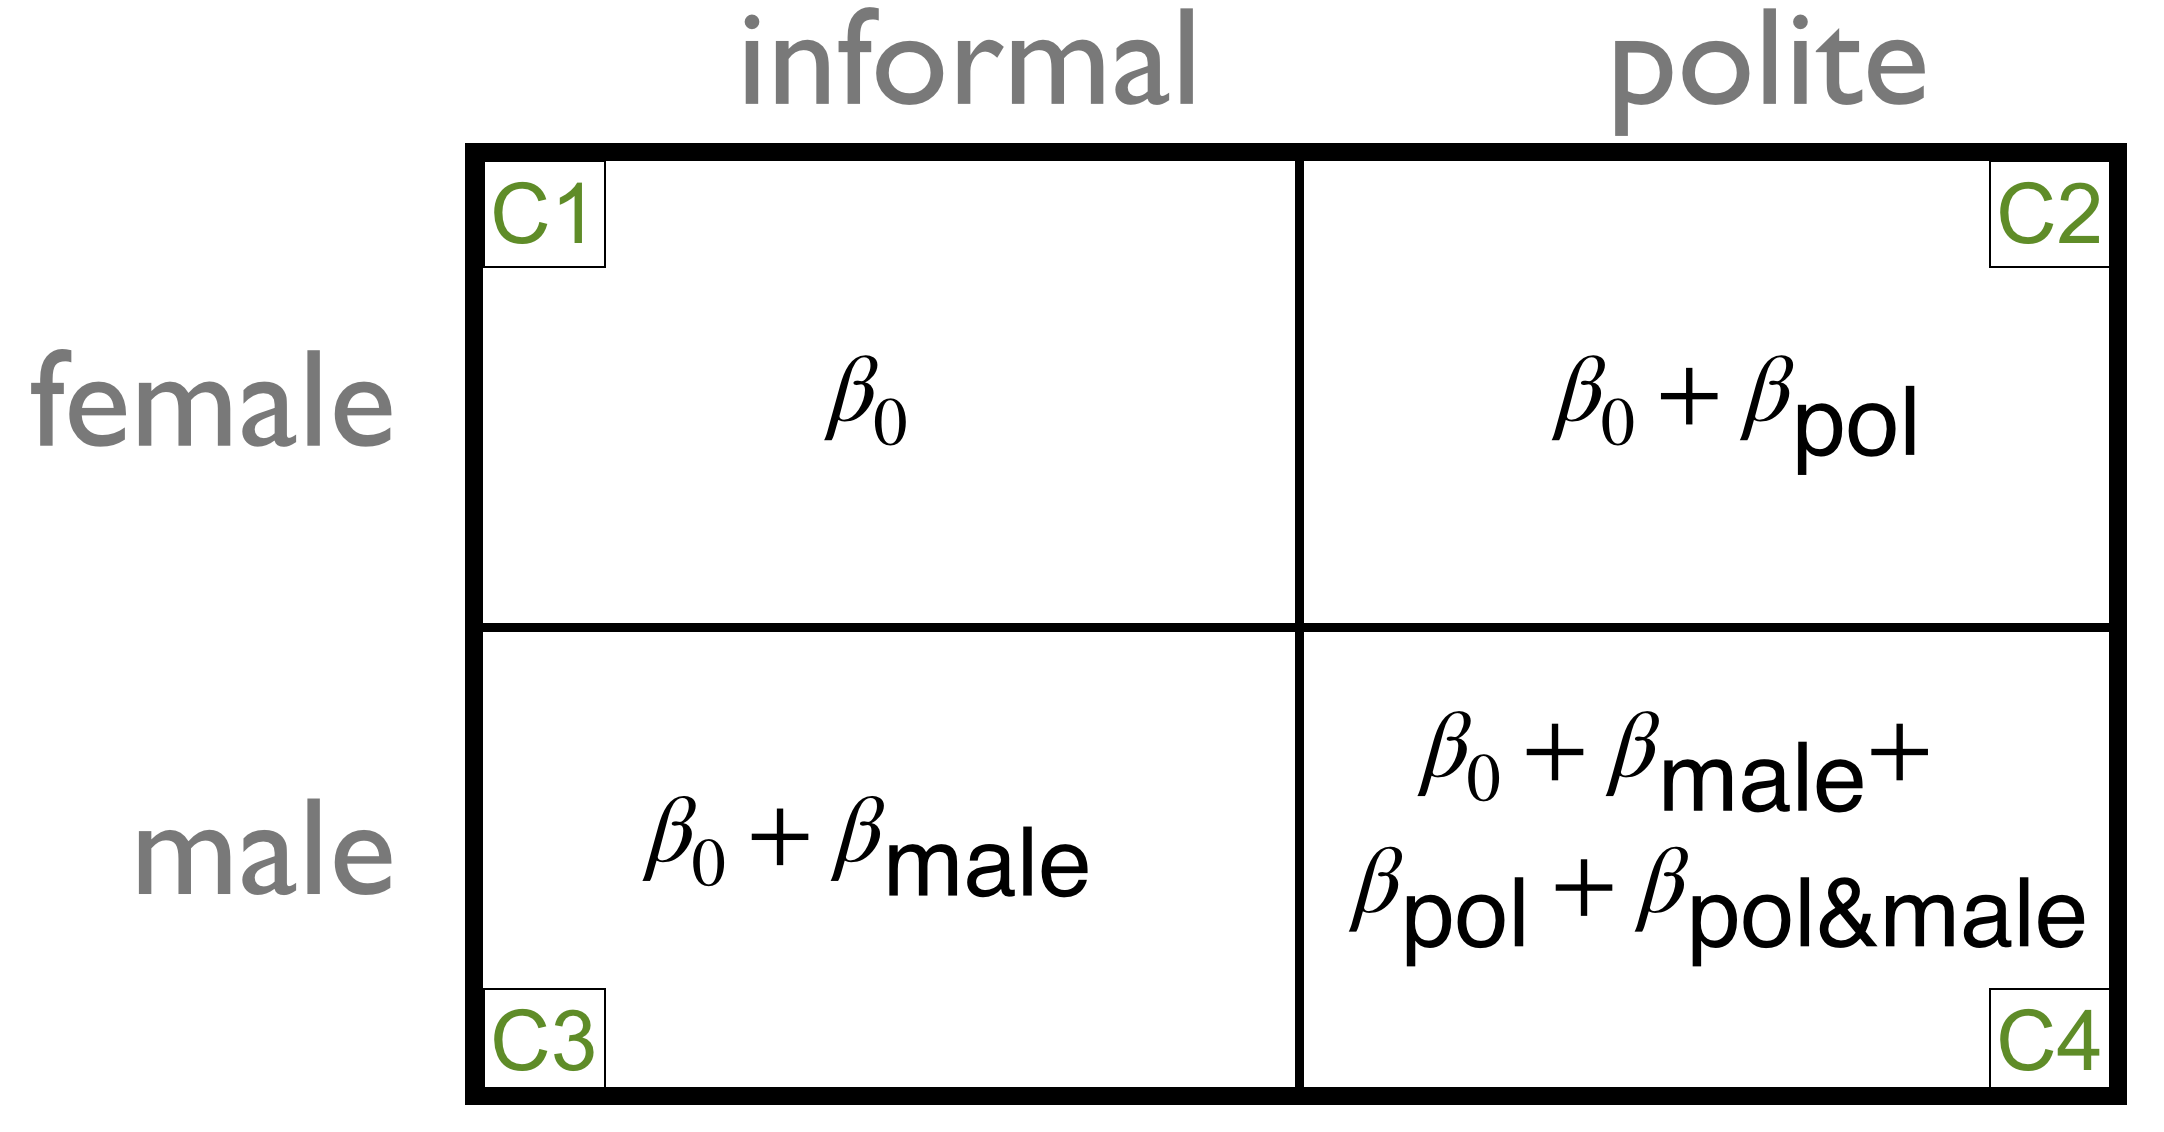
\includegraphics[width = \textwidth]{pics/table_coefficients.png}
    \caption{Coefficients of a dummy-coded regression model for the factorial $2 \times 2$ design.}
    \label{fig:coefficients_table}
\end{figure}

\section{A Bayesian analysis of a (fixed effects) regression model}

Based on our model of how the data was generated, a Bayesian analysis asks: what should we
believe about the values of the coefficients $\beta_0$, $\beta_{\text{pol}}$,
$\beta_{\text{male}}$ and $\beta_{\text{pol\&male}}$?; what values for these parameters are
likely, given the data, the assumed model and our initial beliefs about the parameters?
%
\marginnote{These initial beliefs, also called \textbf{prior beliefs}, are important to get a
  Bayesian analysis off the ground; a circumstance which is discussed controversially. For many
  practical purposes, however, the precise choice of prior is not decisive and tools like the
  \texttt{brms} package which we will use here will default to generically reasonable choices
  of priors for your model (more on this below).}
%
\marginnote{Info Box~1 provides some background on prior beliefs, likelihood function and posterior beliefs.}
%

The R package \texttt{brms} \citep{buerkner2016brms} makes it easy to run Bayesian regression models. It uses much the same formula syntax as related packages for regression analysis. In the case at hand we want to regress the dependent variable \texttt{pitch} against the independent variables \texttt{gender} and \texttt{context} and include their interaction. This model is expressed by the formula:

\begin{minipage}[]{\textwidth}
\begin{lstlisting}[language=R]
# formula for (fixed effects) regression model
formulaFE = pitch ~ gender * context
\end{lstlisting}
\end{minipage}

The Bayesian model can then be fitted with the function \texttt{brm} from the \texttt{brms} package. We only need to specify the formula and supply the data:\marginnote{The \texttt{brms} packages uses probabilistic programming language \texttt{Stan} in the background. Essentially, \texttt{brms} writes Stan code and executes it, which is then translated to C++ (hence the message when you run this code) and used to obtain samples from the posterior distribution, based on an instance of an algorithm called \emph{Hamiltonian Monte Carlo}.}

\begin{minipage}[]{\textwidth}
\begin{lstlisting}[language=R]
# run regression model in brms
modelFE = brm(
  formula = formulaFE,
  data = politedata
)
\end{lstlisting}
\end{minipage}

If you just type in \texttt{modelFE}, you will see a summary of the obtained model fit. It should look (modulo stochastic variation) looks much like the following:

\medskip

\begin{minipage}[]{1.2\textwidth}
\begin{rc}
> modelFE
 Family: gaussian 
  Links: mu = identity; sigma = identity 
Formula: pitch ~ gender * context 
   Data: politedata (Number of observations: 83) 
Samples: 4 chains, each with iter = 2000; warmup = 1000; thin = 1;
         total post-warmup samples = 4000

Population-Level Effects: 
                   Estimate Est.Error l-95% CI u-95% CI Eff.Sample Rhat
Intercept            260.68      8.07   244.99   276.78       2409 1.00
genderM             -116.09     11.44  -138.37   -93.80       2094 1.00
contextpol           -27.38     11.33   -50.01    -5.98       2092 1.00
genderM:contextpol    15.74     16.38   -17.03    49.13       1831 1.00

Family Specific Parameters: 
      Estimate Est.Error l-95% CI u-95% CI Eff.Sample Rhat
sigma    36.15      2.87    30.93    42.40       3652 1.00

Samples were drawn using sampling(NUTS). For each parameter, Eff.Sample 
is a crude measure of effective sample size, and Rhat is the potential 
scale reduction factor on split chains (at convergence, Rhat = 1).
\end{rc}
\end{minipage}

\medskip

This summary tells us a lot. First, we get information about the model and the data used (lines 2--5 above). Lines 6 and 7 tell us about the sampling procedure, e.g., we here have a total of 4000 samples from the posterior distribution, obtained from 4 chains all of which had 2000 iterations but discarded the first 1000 as warmup (more on this below). Lines 9--14 are what is most interesting for evaluating our hypotheses, so we will dwell extensively on them in a moment. Lines 16--18 contain information in a format that is similar to that of lines 9--14, but for a different type of model parameter, namely the standard deviation \texttt{sigma} of the assumed normal distributions (which describe the distribution of measures in each design cell). Finally, lines 20--22 contain general information about the model fit and the information presented in this summary.\marginnote{If the model failed to converge or other problems occurred, you would see an informative message in the last part of this summary.}

Let us now zoom in on the information from lines 9--14 which is theoretically most interesting because this is where we find (partial) answers to the question what we should believe about our research hypotheses. What these lines give us is a table with four rows, each of which corresponds to a parameter in the model, namely the coefficients shown in Figure~\ref{fig:coefficients_table}. The variable \texttt{Intercept} refers to our $\beta_0$, which represents the mean of cell 1 (female speakers in polite contexts; the ``reference cell''). The variable \texttt{genderM} corresponds to our $\beta_{\text{male}}$, \texttt{contextpol} corresponds to our $\beta_{\text{pol}}$, and \texttt{genderM:contextpol} is the interaction term $\beta_{\text{pol\&male}}$. For each of these parameters, the table contains very useful summary statistics based on the samples returned from the model fit. The first column \emph{Estimate} gives the mean of the obtained samples, thereby approximating the mean of the posterior distribution (beliefs we should hold) about each parameter. For example, the parameter \texttt{Intercept} is estimated to have a mean of about $261$, which is (of course) exactly what we calculated as a mean of the data points in cell 1, as shown in Figure~\ref{fig:BasicPlotData_table}. The other columns give further useful information. \emph{Est.Error} is the estimation error, an indication of the certainty we should have about the whole inference procedure. The columns \texttt{l-95\% CI} and \texttt{u-95\% CI} give the lower and upper bound of the \textbf{95\% credible interval} for each parameter, estimated from the posterior samples.
%
\marginnote{Intuitively, the 95\% credible interval is the range of values that we can deem credible enough to care about; the rest is sufficiently unlikely to (perhaps) be ignored, or at least be treated as a different category. Formally, the 95\% credible interval is the set of convex intervals of parameter values such that the probability density over all intervals sums to 0.95 while no parameter value not included in any interval has higher probability density than any point within.}
%
The column \texttt{Eff.Sample}, for efficient samples, gives a rough measure of how many of all the samples we took (4000 in our case) are contributing non-redundant information to our estimation. The higher this number, the better. Finally, \texttt{Rhat} is a measure of whether the samples obtained are likely representative of the true distribution. Concretely, it indicates whether the four chains we ran in parallel all ended up with the same results, so to speak. If this column contains values bigger than 1.1 this is an indication that your model fit has not converged.\marginnote{If your model output indicates non-convergence, you may want to increase the number of samples, but you should also consider the possibility that you are trying to fit a model which cannot be ``trained'' based on the (perhaps insufficient) data and the particular method of posterior sampling. For common regression analyses, this will usually entail considering a simpler model (e.g., with fewer explanatory factors, less (correlated) random effects, etc.)}

For our purposes, the information about 95\% credible intervals is most interesting. Take the parameter \texttt{contextpol}, corresponding to our coefficient $\beta_{\text{pol}}$. The 95\% CI is roughly [-50;-6]. This means that we would take values outside of this interval to be sufficiently unlikely to treat them as ``ignorable''. But that means that we would ignore a very special parameter value for this parameter (including a substantial region around it), namely 0. In intuitive terms, this analysis says that we should not believe that 0 is a credible value for the coefficient $\beta_{\text{pol}}$; rather we should believe that $\beta_{\text{pol}}$ is negative (based on the priors, the regression model and the data; all of which may be critically re-assessed if there are good reasons for it). --- Hurray! This directly addresses our first research hypothesis. In a research paper we could now write: ``Based the regression model, the data suggests that H1 is likely true.''

How likely is it that $\beta_{\text{pol}}$ is smaller than 0? --- It would be even cooler, if we could put a number to it. In fact, we can. To see how this works, let us have a more intimate look at the samples that the \textrm{brm} function returns. We can access the samples of a model fitted with \textrm{brm} with the function \texttt{posterior\_samples}:

\begin{minipage}[]{\textwidth}
\begin{lstlisting}[language=R]
# extract posterior samples 
post_samples_FE = posterior_samples(modelFE)
head(post_samples_FE)
\end{lstlisting}
\end{minipage}

The output of this could look like this:

\medskip

\begin{minipage}[]{1.2\textwidth}
\begin{rc}
> head(post_samples_FE)
  b_Intercept b_genderM b_contextpol b_genderM:contextpol    sigma      lp__
1    255.2955 -106.4147    -24.73881             15.91545 34.24995 -420.0674
2    252.4705 -118.6785    -15.69895             22.73200 35.38918 -421.2423
3    254.0602 -119.7602    -15.87901             15.45185 35.68362 -420.5696
4    270.1344 -114.0217    -33.74421             26.91341 36.25080 -423.0939
5    275.4422 -122.9397    -37.11601             23.48895 37.45709 -422.0191
6    281.3819 -135.4289    -43.38679             25.46482 38.93948 -423.2867
\end{rc}
\end{minipage}

What you see here is the top 6 rows of a data frame with columns for each parameter and 4000 rows, corresponding to each sample of that parameter.
%
\marginnote{The column \texttt{lp\_\_} contains the log-probability of the data for the parameterization in each row. This is useful for model comparison and model criticism but not important for our current adventures.}
%
We can use these samples to produce a density plot. The plot in Figure~\ref{fig:Posteriors_FE} shows, for each of the four main model parameters an estimate of the posterior density. This is, intuitively put, a plot of how much (relative) credence we, as rational agents, should assign to any particular value of each parameter, given the regression model, the specified prior beliefs, and the data. We see that our beliefs concerning plausible values for the mean of cell 1 (female speakers in polite contexts, the reference cell) should hover around 261. We also see that all values that receive substantial probability density for \texttt{contextpol} (our $\beta_{\text{pol}}$) are negative (as captured in the 95\% CI discussed above). 

\begin{figure}
  \centering
  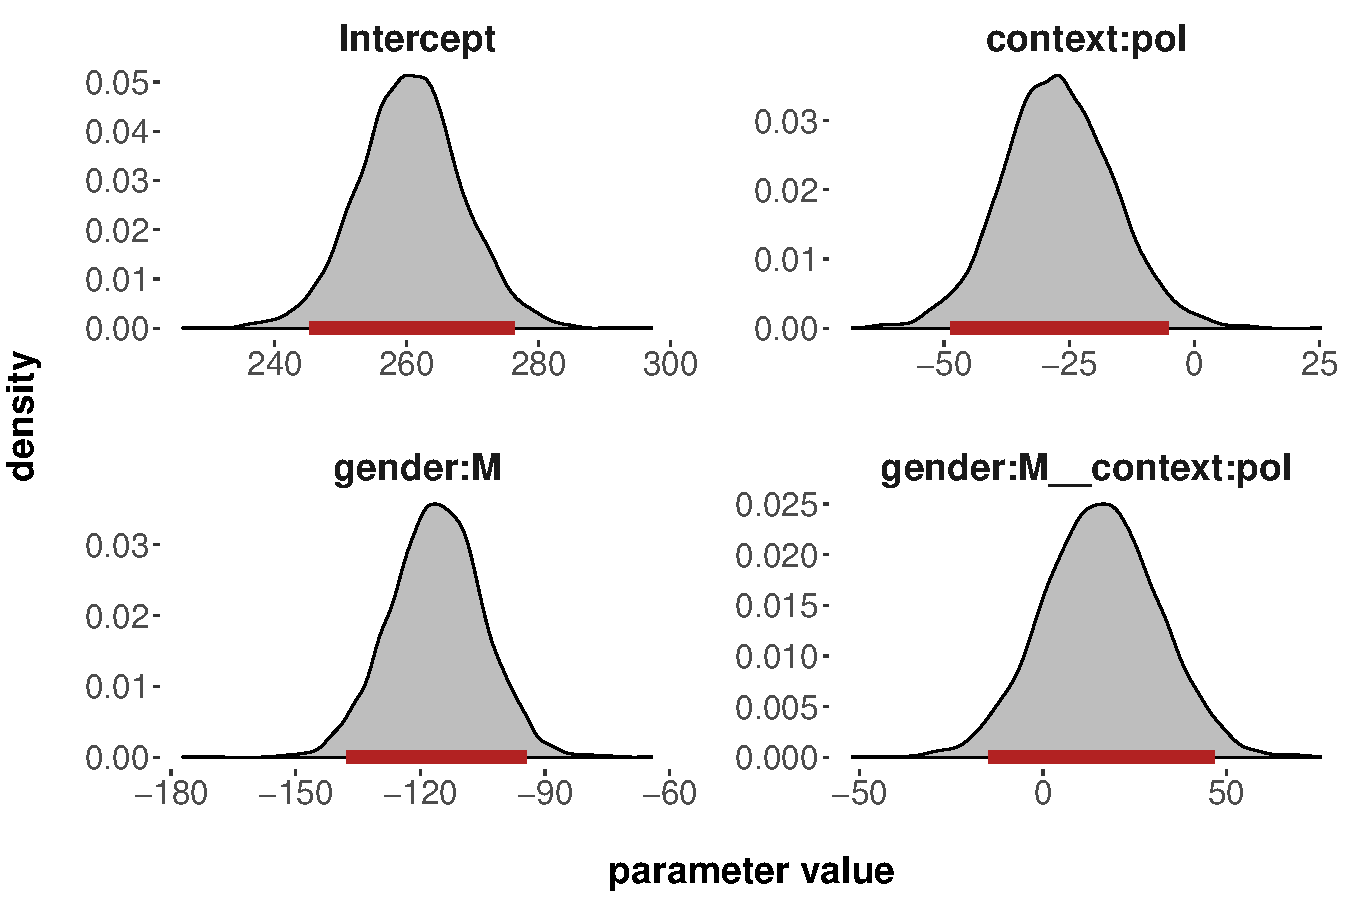
\includegraphics[width=\textwidth]{pics/posterior_density_FE.pdf}
  \caption[Posteriors fixed-effects model]{Posterior density of parameter values in the fixed-effects regression model}
  \label{fig:Posteriors_FE}
\end{figure}

Now, here comes a nice gadget. Based on the samples obtained for \texttt{contextpol} ($\beta_{\text{pol}}$), it is very easy to estimate our belief that $\beta_{\text{pol}}$ is indeed negative. We simply have to calculate the proportion of samples that were negative, that's all. For instance, with the code below, which reveals that the posterior probability, given the data, that $\beta_{\text{pol}} < 0$ is about 0.99275, so very close to certain!  

\begin{minipage}[]{\textwidth}
\begin{lstlisting}[language=R]
# proportion of negative samples for parameter p_contextpol
mean(post_samples_FE$b_contextpol < 0)
\end{lstlisting}
\end{minipage}

In sum, we have seen how to run a Bayesian regression analysis with the \texttt{brms} package and deal with its output. We have also seen that we get output that is interpretable in very terms that also non-statisticians can understand (e.g., ``The probability of H1, given our model, priors, and data, is more than .99''). Unfortunately, what we have not seen yet is what our model and data say about hypotheses 2 or 3.







\bigskip

% \subsection{Priors}

% The syntax of this function should look very familiar to anyone who has worked with (generalized) linear models in R. Now one important difference between traditional frequentist' inferences and a Bayesian framework is that we can take specific prior beliefs about the relationships between dependent and independent variables into account. 

\begin{InfoBox}[t]
\centering
\colorbox{mygray}{\centering
  \begin{minipage}{1.0\textwidth}

    \emph{Bayesian inference: priors, likelihoods and posteriors}
    \medskip

    Jones is a rational scientist. She has recently inherited her grandma's lucky coin. Grandma
    used this coin many times during Jones' childhood to determine whether Jones was allowed a
    sweet or not. Jones suspects that grandma's coin might be a trick coin, but she is not
    sure. She is determined to find out. How? Well, naturally, by rationally updating her
    \emph{prior beliefs} about the coin's bias to obtain a new \emph{posterior belief} based on
    empirical observation (outcomes of coin flips). Central to this updating is Jones'
    \emph{likelihood function}, which encodes how likely each relevant coin bias may have
    generated the observed data. --- Sounds fancifully abstract? It's actially fairly intuitive.
    Consider this example.
    
    \paragraph{Prior beliefs.} Jones initially believes that the coin is either biased towards
    heads or biased towards tails, and that both of these possibilities are equally likely. She
    also believes that, if biased towards heads, the coin is three times more likely to come up
    heads; and that, if biased towards tails, the coin is three times more likely to come up
    tails. Numerically, Jones' \emph{prior beliefs} can be written as, where $\theta \in [0;1]$
    is the coin's bias: $P(\theta = \nicefrac{1}{3}) = \nicefrac{1}{2}$, and $P(\theta =
    \nicefrac{2}{3}) = \nicefrac{1}{2}$.

    \paragraph{Likelihood.} The bias $\theta$ is, by definition, the probability of the coin
    landing heads on the next trial. Let's assume that Jones tosses the coin only once (hm,
    maybe not so rational a scientist after all? or just too busy?). Let $D$ be the set of
    potential outcomes of this experiment, namely $D = \set{\text{heads}, \text{tails}}$. The
    \emph{likelihood function} determines the likelihood of observing each datum $d \in D$ for
    each $\theta$, which in our case is just rather trivial: $P(D = \text{heads} \mid \theta) =
    \theta$ and $P(D = \text{tails} \mid \theta) = 1 - \theta$.

    \paragraph{Posterior beliefs.} Jones observes that the coin landed heads. What should she
    believe now. By \emph{Bayes rule} her posterior beliefs are defined like so:
    \begin{align*}
      P(\theta \mid D = \text{heads}) = \frac{P(\theta) P(D = \text{heads} \mid \theta)}{\sum_{\theta'}P(\theta') P(D = \text{heads} \mid \theta')}
    \end{align*}
    Jones' posterior belief that the coin is twice as likely to land heads is therefore:
    \begin{align*}
      & P(\theta = \nicefrac{2}{3} \mid D = \text{heads}) =  \\
      & \frac{P(\theta = \nicefrac{2}{3}) \ P(D = \text{heads} \mid \theta = \nicefrac{2}{3})}{P(\theta = \nicefrac{2}{3}) \ P(D = \text{heads} \mid \theta = \nicefrac{2}{3}) + P(\theta = \nicefrac{1}{3}) \ P(D = \text{heads} \mid \theta = \nicefrac{1}{3})} = \\
      & \frac{\nicefrac{1}{2} \ \nicefrac{2}{3}}{\nicefrac{1}{2} \ \nicefrac{2}{3} + \nicefrac{1}{2} \ \nicefrac{1}{3}} = \nicefrac{1}{2}
    \end{align*}
    After making her observation, rational Jones believes that the bias towards heads is twice
    more likely than the bias towards tails.
    
  \end{minipage} \par
  } \par
  \begin{center}
    Info Box 1: Priors, likelihood and posteriors in Bayesian inference.
  \end{center}
  % \caption{\label{InfoBox:asymptotic_CIs} Here is my caption}  
\end{InfoBox}



% Priors are subjective pieces of information about your data that you have before analyzing the data. These priors might constrain values that your data can have. For example, mathematically, pitch values  cannot be lower than 0. Practically, human pitch values are within a certain range that is limited by bio mechanical constraints on our laryngeal system. In adults, values beyond, let's say 1000 Hz are very unlikely even when they use falsetto.
% Priors can also express our subjective beliefs about a relationship. For example, knowing what we know about gender differences in pitch, we might be already very certain that female speakers have higher pitch values than male speakers.

% But wait a minute. Subjective beliefs? This is science. We are supposed to be objective, right? You are right. Although, they are cases in which we might want to specify very concrete priors about our data, practically we will restrict ourselves here to what we call weakly informative priors. Weakly informative priors are priors that constrain possible values of a variable (e.g. possible pitch values). These priors are also called regularizing priors, as they help the statistical model to converge on reasonable estimates. But these priors are also agnostic about possible relationships between variables. 



% \tr{Below is stuff to mention when we transition to hierarchical models}. 

% These mean values, however, are a very poor and abstract representation of all the pitch values that we have recorded. Different speakers have very different voice pitch ranges. Likewise, speakers are not machines. There is a substantial variability in how a single speaker pronounces an utterance. So we expect some variability here. Likewise,
% different scenarios might elicit very different pitch values due idiosyncratic aspects of the scenario that are not captured by our independent variables. 

% In our study, we took multiple measures per speaker. That is, each subject gave multiple polite responses and multiple informal responses. 
% Individual responses from one subject are thus dependent. Also, we took multiple measures per scenario, as each scenario was produced by all speakers. This introduces, again, dependencies between data points. These dependencies need to be taken into account when we try to estimate differences between groups.









\printbibliography[heading=bibintoc]

\end{document}
